\begin{figure}[H]
\begin{center}
\centerline{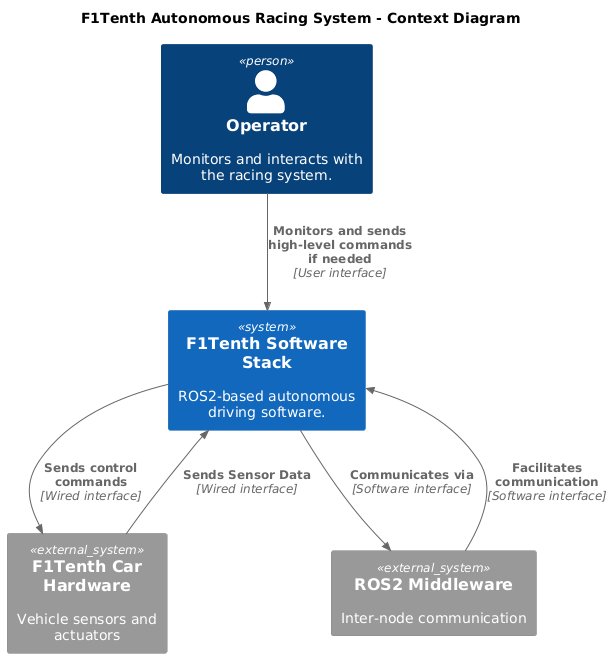
\includegraphics[width=\columnwidth]{Context.png}}
\caption{Context diagram (C4 Level 1) of the used software architecture}
\label{fig:arch-context}
\end{center}
\end{figure}
The software architecture is based on a software stack which uses the ROS2 Middleware to facilitate communication and sends drive commands to as well as receives sensor data from a provided F1Tenth Hardware Stack as seen in Figure~\ref{fig:arch-context}.
\begin{figure}[H]
\begin{center}
\centerline{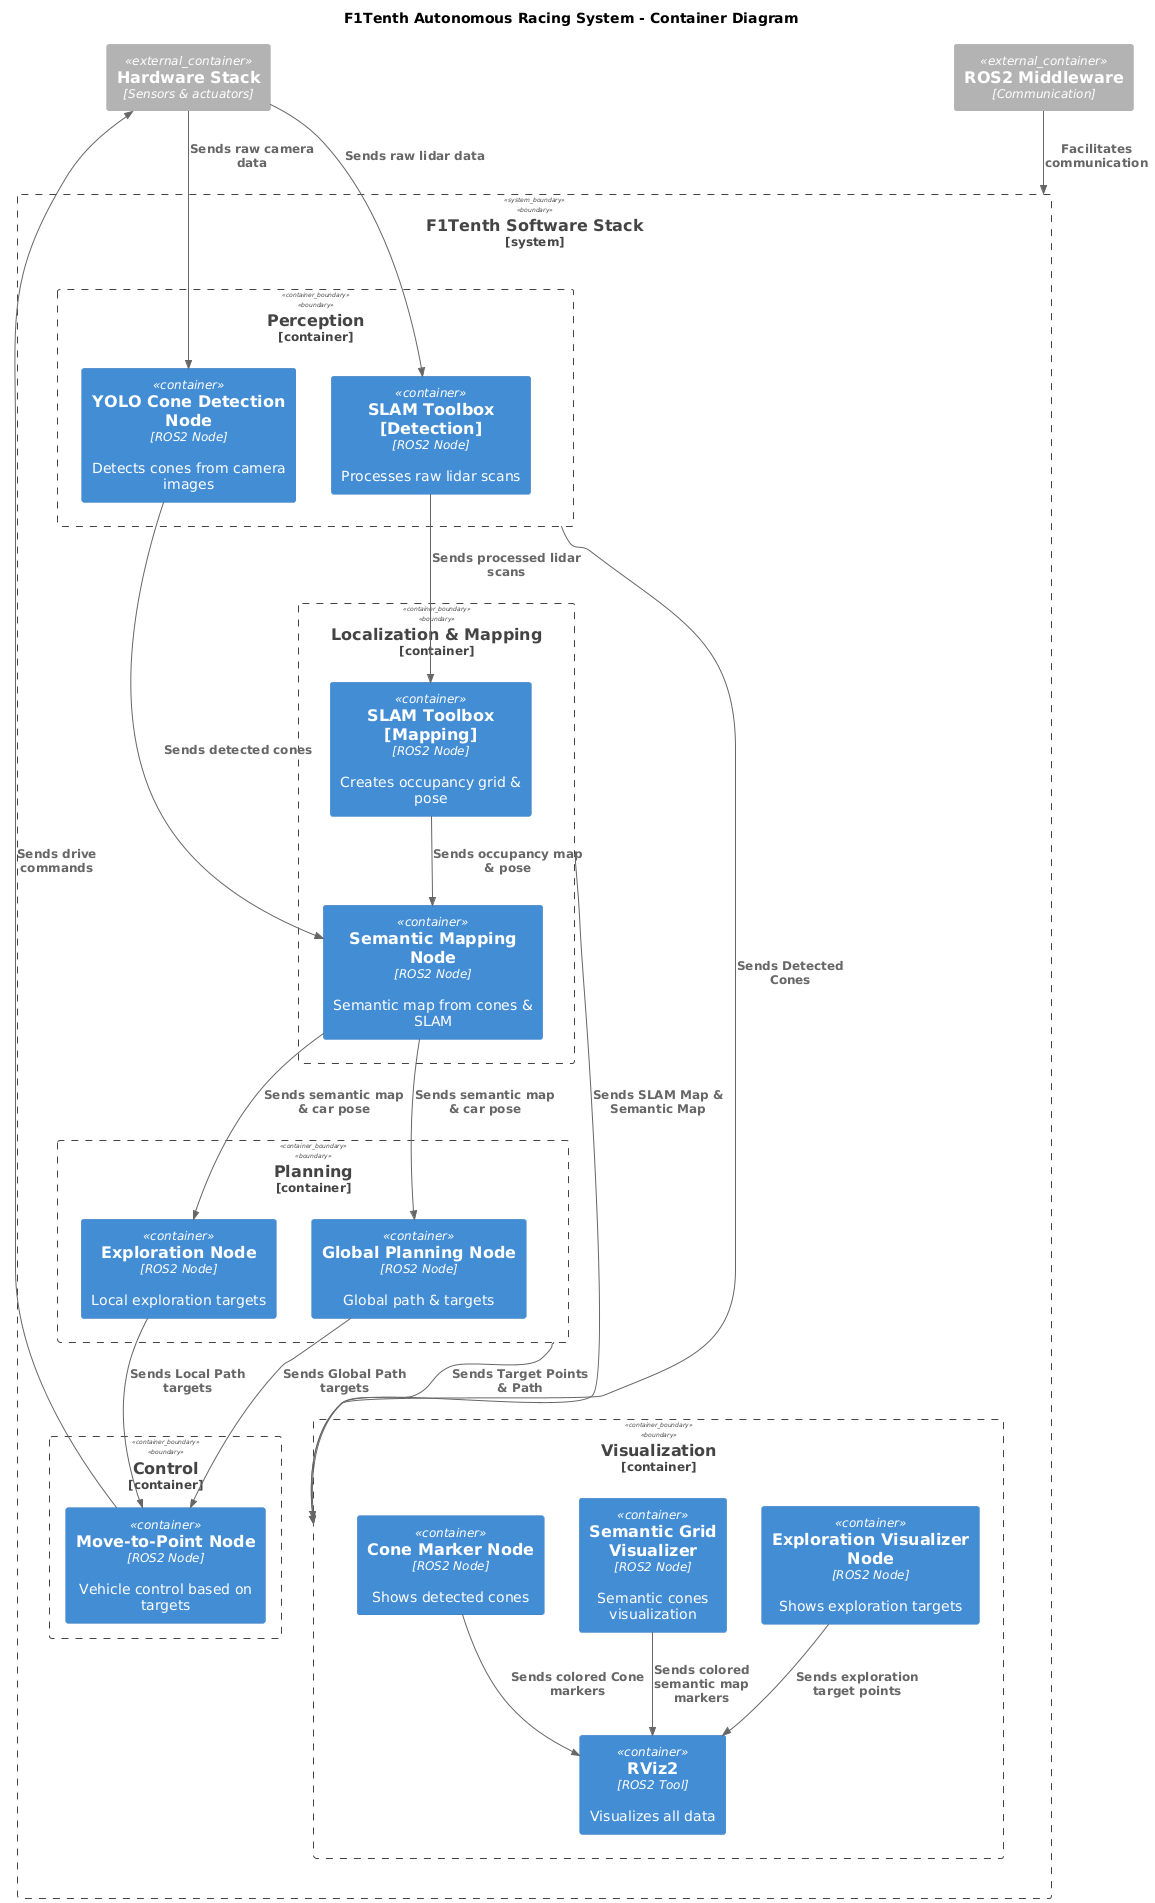
\includegraphics[width=0.85\columnwidth]{Container.png}}
\caption{Container diagram (C4 Level 2) of the used software architecture}
\label{fig:arch-container}
\end{center}
\end{figure}
As shown in Figure~\ref{fig:arch-container}, the autonomous vehicle system is divided into several interconnected modules that ensure efficient perception, localization \& mapping, planning and control. 
The perception system includes cone detection, which is performed by a YOLO-based node that uses a trained deep learning model to identify cones in the camera image.
Here, SLAM Toolbox is used to interpret the LIDAR sensor data.
\newline
In the localization \& mapping module, the LIDAR-based map and corrected pose information from the SLAM Toolbox, as well as the cone detections from the perception module are fused in a Semantic Mapping Node. The resulting semantic map, which now includes cone color information is essential for the path planning. 
\newline
The path planning module generates an optimal trajectory that ensures that the vehicle navigates the track efficiently. It processes environmental information, vehicle dynamics, and track constraints to determine a feasible and optimized driving path.
The planning process consists of two stages. Initially, the system explores the track to gather key information about the environment and construct a representation of the drivable space. Once sufficient data is collected, the module transitions to a global planning mode, where it optimizes the trajectory based on the recorded driving path to ensure smooth navigation.
\newline
Target points calculated by the planning module are sent to the control module to be further processed into drive commands for our hardware stack.
\newline
Additionally, a visualization module gets intermittent outputs from each module to visualize calculated perception detections, maps and paths via RViz2.\\